\documentclass[1p]{elsarticle_modified}
%\bibliographystyle{elsarticle-num}

%\usepackage[colorlinks]{hyperref}
%\usepackage{abbrmath_seonhwa} %\Abb, \Ascr, \Acal ,\Abf, \Afrak
\usepackage{amsfonts}
\usepackage{amssymb}
\usepackage{amsmath}
\usepackage{amsthm}
\usepackage{scalefnt}
\usepackage{amsbsy}
\usepackage{kotex}
\usepackage{caption}
\usepackage{subfig}
\usepackage{color}
\usepackage{graphicx}
\usepackage{xcolor} %% white, black, red, green, blue, cyan, magenta, yellow
\usepackage{float}
\usepackage{setspace}
\usepackage{hyperref}

\usepackage{tikz}
\usetikzlibrary{arrows}

\usepackage{multirow}
\usepackage{array} % fixed length table
\usepackage{hhline}

%%%%%%%%%%%%%%%%%%%%%
\makeatletter
\renewcommand*\env@matrix[1][\arraystretch]{%
	\edef\arraystretch{#1}%
	\hskip -\arraycolsep
	\let\@ifnextchar\new@ifnextchar
	\array{*\c@MaxMatrixCols c}}
\makeatother %https://tex.stackexchange.com/questions/14071/how-can-i-increase-the-line-spacing-in-a-matrix
%%%%%%%%%%%%%%%

\usepackage[normalem]{ulem}

\newcommand{\msout}[1]{\ifmmode\text{\sout{\ensuremath{#1}}}\else\sout{#1}\fi}
%SOURCE: \msout is \stkout macro in https://tex.stackexchange.com/questions/20609/strikeout-in-math-mode

\newcommand{\cancel}[1]{
	\ifmmode
	{\color{red}\msout{#1}}
	\else
	{\color{red}\sout{#1}}
	\fi
}

\newcommand{\add}[1]{
	{\color{blue}\uwave{#1}}
}

\newcommand{\replace}[2]{
	\ifmmode
	{\color{red}\msout{#1}}{\color{blue}\uwave{#2}}
	\else
	{\color{red}\sout{#1}}{\color{blue}\uwave{#2}}
	\fi
}

\newcommand{\Sol}{\mathcal{S}} %segment
\newcommand{\D}{D} %diagram
\newcommand{\A}{\mathcal{A}} %arc


%%%%%%%%%%%%%%%%%%%%%%%%%%%%%5 test

\def\sl{\operatorname{\textup{SL}}(2,\Cbb)}
\def\psl{\operatorname{\textup{PSL}}(2,\Cbb)}
\def\quan{\mkern 1mu \triangleright \mkern 1mu}

\theoremstyle{definition}
\newtheorem{thm}{Theorem}[section]
\newtheorem{prop}[thm]{Proposition}
\newtheorem{lem}[thm]{Lemma}
\newtheorem{ques}[thm]{Question}
\newtheorem{cor}[thm]{Corollary}
\newtheorem{defn}[thm]{Definition}
\newtheorem{exam}[thm]{Example}
\newtheorem{rmk}[thm]{Remark}
\newtheorem{alg}[thm]{Algorithm}

\newcommand{\I}{\sqrt{-1}}
\begin{document}

%\begin{frontmatter}
%
%\title{Boundary parabolic representations of knots up to 8 crossings}
%
%%% Group authors per affiliation:
%\author{Yunhi Cho} 
%\address{Department of Mathematics, University of Seoul, Seoul, Korea}
%\ead{yhcho@uos.ac.kr}
%
%
%\author{Seonhwa Kim} %\fnref{s_kim}}
%\address{Center for Geometry and Physics, Institute for Basic Science, Pohang, 37673, Korea}
%\ead{ryeona17@ibs.re.kr}
%
%\author{Hyuk Kim}
%\address{Department of Mathematical Sciences, Seoul National University, Seoul 08826, Korea}
%\ead{hyukkim@snu.ac.kr}
%
%\author{Seokbeom Yoon}
%\address{Department of Mathematical Sciences, Seoul National University, Seoul, 08826,  Korea}
%\ead{sbyoon15@snu.ac.kr}
%
%\begin{abstract}
%We find all boundary parabolic representation of knots up to 8 crossings.
%
%\end{abstract}
%\begin{keyword}
%    \MSC[2010] 57M25 
%\end{keyword}
%
%\end{frontmatter}

%\linenumbers
%\tableofcontents
%
\newcommand\colored[1]{\textcolor{white}{\rule[-0.35ex]{0.8em}{1.4ex}}\kern-0.8em\color{red} #1}%
%\newcommand\colored[1]{\textcolor{white}{ #1}\kern-2.17ex	\textcolor{white}{ #1}\kern-1.81ex	\textcolor{white}{ #1}\kern-2.15ex\color{red}#1	}

{\Large $\underline{12a_{0099}~(K12a_{0099})}$}

\setlength{\tabcolsep}{10pt}
\renewcommand{\arraystretch}{1.6}
\vspace{1cm}\begin{tabular}{m{100pt}>{\centering\arraybackslash}m{274pt}}
\multirow{5}{120pt}{
	\centering
	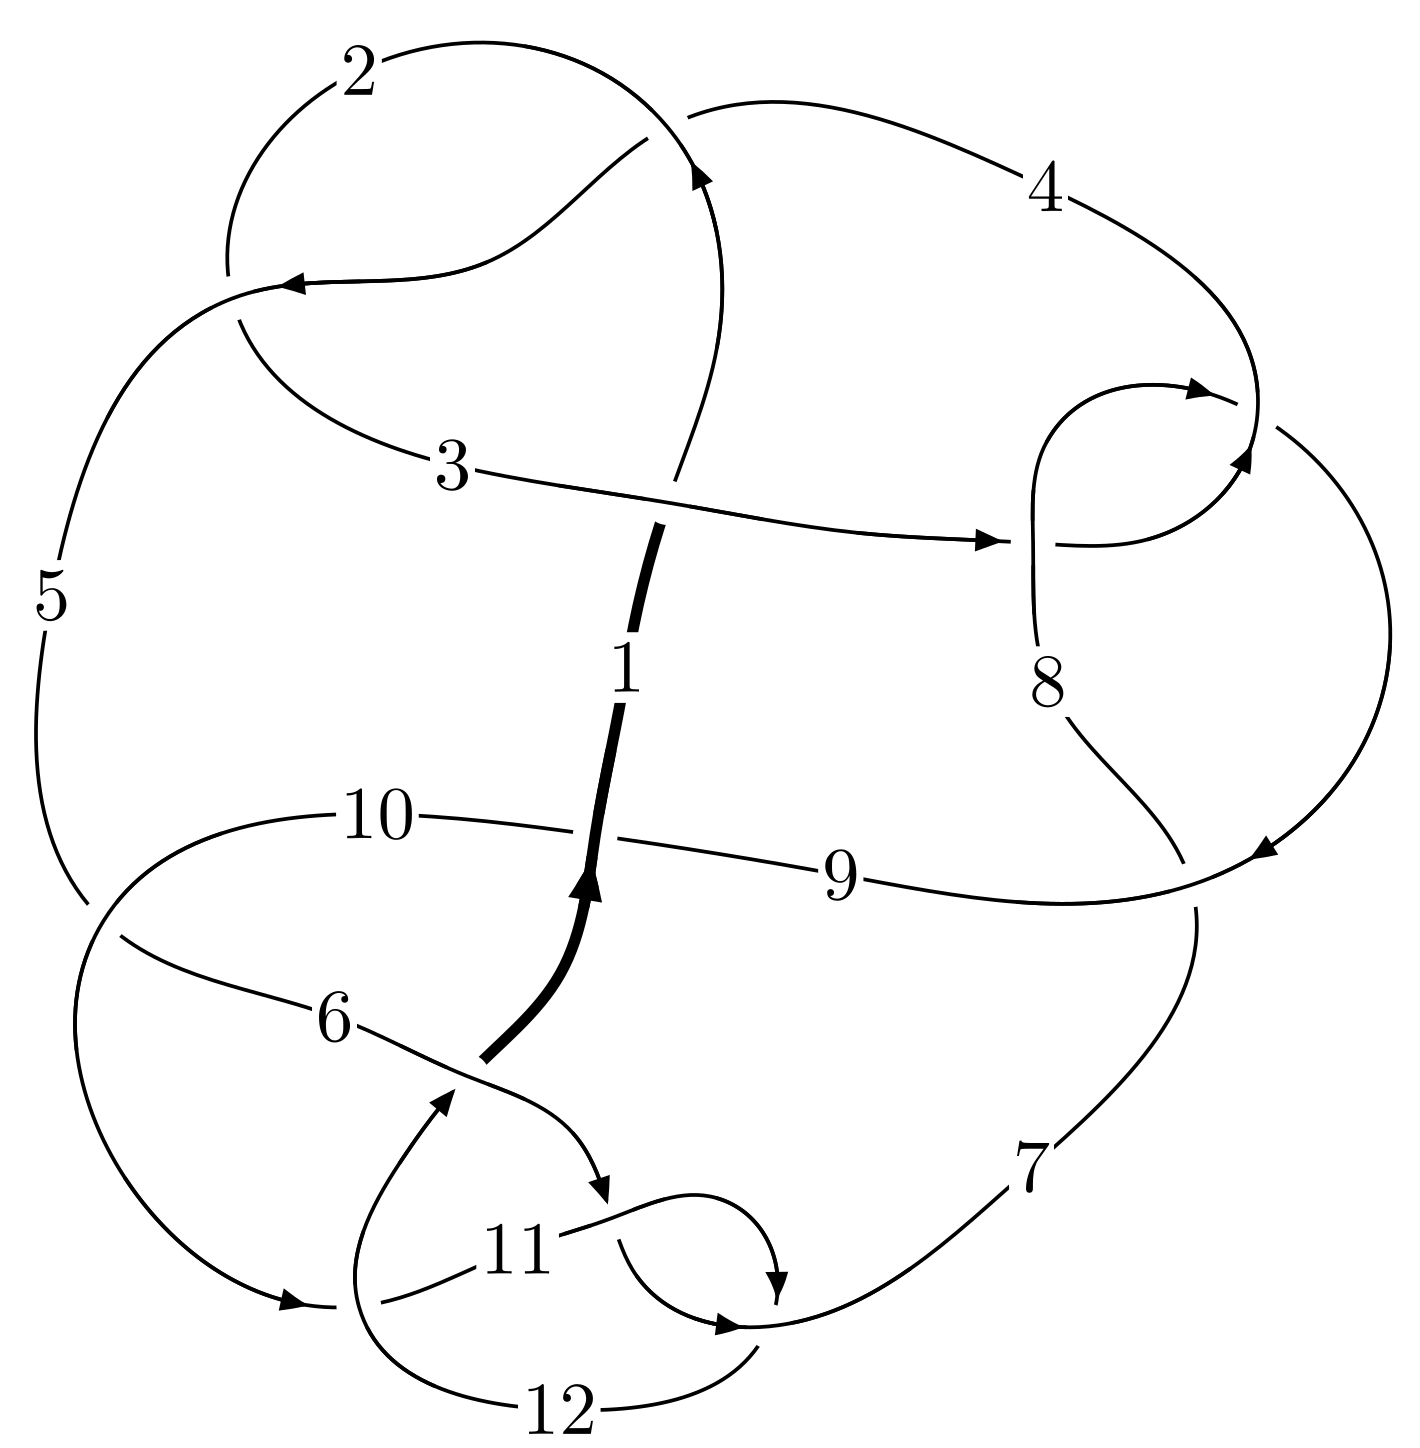
\includegraphics[width=112pt]{../../../GIT/diagram.site/Diagrams/png/900_12a_0099.png}\\
\ \ \ A knot diagram\footnotemark}&
\allowdisplaybreaks
\textbf{Linearized knot diagam} \\
\cline{2-2}
 &
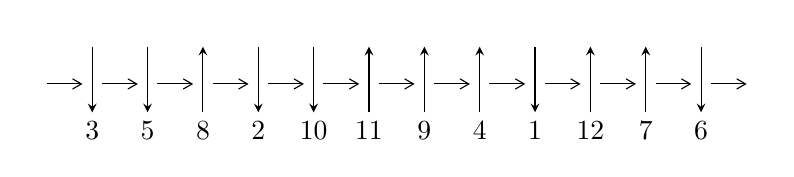
\begin{tikzpicture}[x=20pt, y=17pt]
	% nodes
	\node (C0) at (0, 0) {};
	\node (C1) at (1, 0) {};
	\node (C1U) at (1, +1) {};
	\node (C1D) at (1, -1) {3};

	\node (C2) at (2, 0) {};
	\node (C2U) at (2, +1) {};
	\node (C2D) at (2, -1) {5};

	\node (C3) at (3, 0) {};
	\node (C3U) at (3, +1) {};
	\node (C3D) at (3, -1) {8};

	\node (C4) at (4, 0) {};
	\node (C4U) at (4, +1) {};
	\node (C4D) at (4, -1) {2};

	\node (C5) at (5, 0) {};
	\node (C5U) at (5, +1) {};
	\node (C5D) at (5, -1) {10};

	\node (C6) at (6, 0) {};
	\node (C6U) at (6, +1) {};
	\node (C6D) at (6, -1) {11};

	\node (C7) at (7, 0) {};
	\node (C7U) at (7, +1) {};
	\node (C7D) at (7, -1) {9};

	\node (C8) at (8, 0) {};
	\node (C8U) at (8, +1) {};
	\node (C8D) at (8, -1) {4};

	\node (C9) at (9, 0) {};
	\node (C9U) at (9, +1) {};
	\node (C9D) at (9, -1) {1};

	\node (C10) at (10, 0) {};
	\node (C10U) at (10, +1) {};
	\node (C10D) at (10, -1) {12};

	\node (C11) at (11, 0) {};
	\node (C11U) at (11, +1) {};
	\node (C11D) at (11, -1) {7};

	\node (C12) at (12, 0) {};
	\node (C12U) at (12, +1) {};
	\node (C12D) at (12, -1) {6};
	\node (C13) at (13, 0) {};

	% arrows
	\draw[->,>={angle 60}]
	(C0) edge (C1) (C1) edge (C2) (C2) edge (C3) (C3) edge (C4) (C4) edge (C5) (C5) edge (C6) (C6) edge (C7) (C7) edge (C8) (C8) edge (C9) (C9) edge (C10) (C10) edge (C11) (C11) edge (C12) (C12) edge (C13) ;	\draw[->,>=stealth]
	(C1U) edge (C1D) (C2U) edge (C2D) (C3D) edge (C3U) (C4U) edge (C4D) (C5U) edge (C5D) (C6D) edge (C6U) (C7D) edge (C7U) (C8D) edge (C8U) (C9U) edge (C9D) (C10D) edge (C10U) (C11D) edge (C11U) (C12U) edge (C12D) ;
	\end{tikzpicture} \\
\hhline{~~} \\& 
\textbf{Solving Sequence} \\ \cline{2-2} 
 &
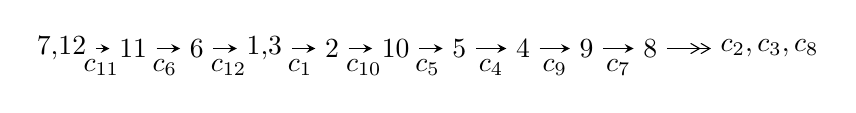
\begin{tikzpicture}[x=23pt, y=7pt]
	% node
	\node (A0) at (-1/8, 0) {7,12};
	\node (A1) at (1, 0) {11};
	\node (A2) at (2, 0) {6};
	\node (A3) at (49/16, 0) {1,3};
	\node (A4) at (33/8, 0) {2};
	\node (A5) at (41/8, 0) {10};
	\node (A6) at (49/8, 0) {5};
	\node (A7) at (57/8, 0) {4};
	\node (A8) at (65/8, 0) {9};
	\node (A9) at (73/8, 0) {8};
	\node (C1) at (1/2, -1) {$c_{11}$};
	\node (C2) at (3/2, -1) {$c_{6}$};
	\node (C3) at (5/2, -1) {$c_{12}$};
	\node (C4) at (29/8, -1) {$c_{1}$};
	\node (C5) at (37/8, -1) {$c_{10}$};
	\node (C6) at (45/8, -1) {$c_{5}$};
	\node (C7) at (53/8, -1) {$c_{4}$};
	\node (C8) at (61/8, -1) {$c_{9}$};
	\node (C9) at (69/8, -1) {$c_{7}$};
	\node (A10) at (11, 0) {$c_{2},c_{3},c_{8}$};

	% edge
	\draw[->,>=stealth]	
	(A0) edge (A1) (A1) edge (A2) (A2) edge (A3) (A3) edge (A4) (A4) edge (A5) (A5) edge (A6) (A6) edge (A7) (A7) edge (A8) (A8) edge (A9) ;
	\draw[->>,>={angle 60}]	
	(A9) edge (A10);
\end{tikzpicture} \\ 

\end{tabular} \\

\footnotetext{
The image of knot diagram is generated by the software ``\textbf{Draw programme}" developed by Andrew Bartholomew(\url{http://www.layer8.co.uk/maths/draw/index.htm\#Running-draw}), where we modified some parts for our purpose(\url{https://github.com/CATsTAILs/LinksPainter}).
}\phantom \\ \newline 
\centering \textbf{Ideals for irreducible components\footnotemark of $X_{\text{par}}$} 
 
\begin{align*}
I^u_{1}&=\langle 
u^{113}+u^{112}+\cdots+b+u,\;- u^{113}- u^{112}+\cdots+a+u,\;u^{114}+2 u^{113}+\cdots+3 u+1\rangle \\
I^u_{2}&=\langle 
u^5+u^4- u^3- u^2+b,\;a,\;u^6+u^5- u^4-2 u^3+u+1\rangle \\
\\
\end{align*}
\raggedright * 2 irreducible components of $\dim_{\mathbb{C}}=0$, with total 120 representations.\\
\footnotetext{All coefficients of polynomials are rational numbers. But the coefficients are sometimes approximated in decimal forms when there is not enough margin.}
\newpage
\renewcommand{\arraystretch}{1}
\centering \section*{I. $I^u_{1}= \langle u^{113}+u^{112}+\cdots+b+u,\;- u^{113}- u^{112}+\cdots+a+u,\;u^{114}+2 u^{113}+\cdots+3 u+1 \rangle$}
\flushleft \textbf{(i) Arc colorings}\\
\begin{tabular}{m{7pt} m{180pt} m{7pt} m{180pt} }
\flushright $a_{7}=$&$\begin{pmatrix}0\\u\end{pmatrix}$ \\
\flushright $a_{12}=$&$\begin{pmatrix}1\\0\end{pmatrix}$ \\
\flushright $a_{11}=$&$\begin{pmatrix}1\\u^2\end{pmatrix}$ \\
\flushright $a_{6}=$&$\begin{pmatrix}- u\\- u^3+u\end{pmatrix}$ \\
\flushright $a_{1}=$&$\begin{pmatrix}u^4- u^2+1\\u^6-2 u^4+u^2\end{pmatrix}$ \\
\flushright $a_{3}=$&$\begin{pmatrix}u^{113}+u^{112}+\cdots+2 u^3- u\\- u^{113}- u^{112}+\cdots-2 u^2- u\end{pmatrix}$ \\
\flushright $a_{2}=$&$\begin{pmatrix}- u^{59}+14 u^{57}+\cdots-2 u^2-2 u\\- u^{112}- u^{111}+\cdots- u^2- u\end{pmatrix}$ \\
\flushright $a_{10}=$&$\begin{pmatrix}- u^2+1\\u^2\end{pmatrix}$ \\
\flushright $a_{5}=$&$\begin{pmatrix}- u^7+2 u^5-2 u^3\\u^7- u^5+u\end{pmatrix}$ \\
\flushright $a_{4}=$&$\begin{pmatrix}- u^{113}- u^{112}+\cdots-3 u-1\\u^{113}- u^{112}+\cdots+2 u^5+u^3\end{pmatrix}$ \\
\flushright $a_{9}=$&$\begin{pmatrix}u^{12}-3 u^{10}+5 u^8-4 u^6+2 u^4- u^2+1\\u^{14}-4 u^{12}+7 u^{10}-6 u^8+2 u^6+u^2\end{pmatrix}$ \\
\flushright $a_{8}=$&$\begin{pmatrix}u^{25}-6 u^{23}+\cdots-2 u^3+u\\u^{27}-7 u^{25}+\cdots+u^3+u\end{pmatrix}$\\&\end{tabular}
\flushleft \textbf{(ii) Obstruction class $= -1$}\\~\\
\flushleft \textbf{(iii) Cusp Shapes $= 12 u^{113}+14 u^{112}+\cdots+20 u+10$}\\~\\
\newpage\renewcommand{\arraystretch}{1}
\flushleft \textbf{(iv) u-Polynomials at the component}\newline \\
\begin{tabular}{m{50pt}|m{274pt}}
Crossings & \hspace{64pt}u-Polynomials at each crossing \\
\hline $$\begin{aligned}c_{1}\end{aligned}$$&$\begin{aligned}
&u^{114}+61 u^{113}+\cdots+8 u+1
\end{aligned}$\\
\hline $$\begin{aligned}c_{2},c_{4}\end{aligned}$$&$\begin{aligned}
&u^{114}-7 u^{113}+\cdots-8 u+1
\end{aligned}$\\
\hline $$\begin{aligned}c_{3},c_{8}\end{aligned}$$&$\begin{aligned}
&u^{114}+u^{113}+\cdots-64 u+64
\end{aligned}$\\
\hline $$\begin{aligned}c_{5}\end{aligned}$$&$\begin{aligned}
&u^{114}+2 u^{113}+\cdots-60045 u+5113
\end{aligned}$\\
\hline $$\begin{aligned}c_{6},c_{11}\end{aligned}$$&$\begin{aligned}
&u^{114}-2 u^{113}+\cdots-3 u+1
\end{aligned}$\\
\hline $$\begin{aligned}c_{7}\end{aligned}$$&$\begin{aligned}
&u^{114}-39 u^{113}+\cdots-114688 u+4096
\end{aligned}$\\
\hline $$\begin{aligned}c_{9}\end{aligned}$$&$\begin{aligned}
&u^{114}-14 u^{113}+\cdots-4339 u+349
\end{aligned}$\\
\hline $$\begin{aligned}c_{10}\end{aligned}$$&$\begin{aligned}
&u^{114}-54 u^{113}+\cdots+u+1
\end{aligned}$\\
\hline $$\begin{aligned}c_{12}\end{aligned}$$&$\begin{aligned}
&u^{114}-6 u^{113}+\cdots-13547 u+1585
\end{aligned}$\\
\hline
\end{tabular}\\~\\
\newpage\renewcommand{\arraystretch}{1}
\flushleft \textbf{(v) Riley Polynomials at the component}\newline \\
\begin{tabular}{m{50pt}|m{274pt}}
Crossings & \hspace{64pt}Riley Polynomials at each crossing \\
\hline $$\begin{aligned}c_{1}\end{aligned}$$&$\begin{aligned}
&y^{114}-9 y^{113}+\cdots-16 y+1
\end{aligned}$\\
\hline $$\begin{aligned}c_{2},c_{4}\end{aligned}$$&$\begin{aligned}
&y^{114}-61 y^{113}+\cdots-8 y+1
\end{aligned}$\\
\hline $$\begin{aligned}c_{3},c_{8}\end{aligned}$$&$\begin{aligned}
&y^{114}-39 y^{113}+\cdots-114688 y+4096
\end{aligned}$\\
\hline $$\begin{aligned}c_{5}\end{aligned}$$&$\begin{aligned}
&y^{114}-30 y^{113}+\cdots-2610115671 y+26142769
\end{aligned}$\\
\hline $$\begin{aligned}c_{6},c_{11}\end{aligned}$$&$\begin{aligned}
&y^{114}-54 y^{113}+\cdots+y+1
\end{aligned}$\\
\hline $$\begin{aligned}c_{7}\end{aligned}$$&$\begin{aligned}
&y^{114}+61 y^{113}+\cdots-486539264 y+16777216
\end{aligned}$\\
\hline $$\begin{aligned}c_{9}\end{aligned}$$&$\begin{aligned}
&y^{114}+6 y^{113}+\cdots+2982089 y+121801
\end{aligned}$\\
\hline $$\begin{aligned}c_{10}\end{aligned}$$&$\begin{aligned}
&y^{114}+14 y^{113}+\cdots+9 y+1
\end{aligned}$\\
\hline $$\begin{aligned}c_{12}\end{aligned}$$&$\begin{aligned}
&y^{114}+26 y^{113}+\cdots+126216321 y+2512225
\end{aligned}$\\
\hline
\end{tabular}\\~\\
\newpage\flushleft \textbf{(vi) Complex Volumes and Cusp Shapes}
$$\begin{array}{c|c|c}  
\text{Solutions to }I^u_{1}& \I (\text{vol} + \sqrt{-1}CS) & \text{Cusp shape}\\
 \hline 
\begin{aligned}
u &= -0.802895 + 0.478978 I \\
a &= \phantom{-}0.648034 + 0.661607 I \\
b &= \phantom{-}1.081410 - 0.794048 I\end{aligned}
 & \phantom{-}1.73492 + 0.06692 I & \phantom{-0.000000 } 0 \\ \hline\begin{aligned}
u &= -0.802895 - 0.478978 I \\
a &= \phantom{-}0.648034 - 0.661607 I \\
b &= \phantom{-}1.081410 + 0.794048 I\end{aligned}
 & \phantom{-}1.73492 - 0.06692 I & \phantom{-0.000000 } 0 \\ \hline\begin{aligned}
u &= -0.621442 + 0.675702 I \\
a &= -2.36173 - 0.66170 I \\
b &= \phantom{-}0.38621 + 2.96578 I\end{aligned}
 & -4.92367 - 10.31030 I & \phantom{-0.000000 } 0 \\ \hline\begin{aligned}
u &= -0.621442 - 0.675702 I \\
a &= -2.36173 + 0.66170 I \\
b &= \phantom{-}0.38621 - 2.96578 I\end{aligned}
 & -4.92367 + 10.31030 I & \phantom{-0.000000 } 0 \\ \hline\begin{aligned}
u &= -1.075240 + 0.161250 I \\
a &= \phantom{-}0.221621 - 0.332650 I \\
b &= \phantom{-}0.442594 + 1.153370 I\end{aligned}
 & -0.60639 - 3.57403 I & \phantom{-0.000000 } 0 \\ \hline\begin{aligned}
u &= -1.075240 - 0.161250 I \\
a &= \phantom{-}0.221621 + 0.332650 I \\
b &= \phantom{-}0.442594 - 1.153370 I\end{aligned}
 & -0.60639 + 3.57403 I & \phantom{-0.000000 } 0 \\ \hline\begin{aligned}
u &= -1.071530 + 0.244885 I \\
a &= \phantom{-}1.110960 - 0.154532 I \\
b &= -0.631824 - 0.105891 I\end{aligned}
 & \phantom{-}2.19637 - 0.24343 I & \phantom{-0.000000 } 0 \\ \hline\begin{aligned}
u &= -1.071530 - 0.244885 I \\
a &= \phantom{-}1.110960 + 0.154532 I \\
b &= -0.631824 + 0.105891 I\end{aligned}
 & \phantom{-}2.19637 + 0.24343 I & \phantom{-0.000000 } 0 \\ \hline\begin{aligned}
u &= -0.886335 + 0.160699 I \\
a &= \phantom{-}0.590127 + 0.021652 I \\
b &= \phantom{-}0.224427 - 0.276342 I\end{aligned}
 & \phantom{-}1.57240 - 0.20684 I & \phantom{-0.000000 } 0 \\ \hline\begin{aligned}
u &= -0.886335 - 0.160699 I \\
a &= \phantom{-}0.590127 - 0.021652 I \\
b &= \phantom{-}0.224427 + 0.276342 I\end{aligned}
 & \phantom{-}1.57240 + 0.20684 I & \phantom{-0.000000 } 0\\
 \hline 
 \end{array}$$\newpage$$\begin{array}{c|c|c}  
\text{Solutions to }I^u_{1}& \I (\text{vol} + \sqrt{-1}CS) & \text{Cusp shape}\\
 \hline 
\begin{aligned}
u &= -0.615559 + 0.654054 I \\
a &= \phantom{-}1.149110 + 0.493027 I \\
b &= \phantom{-}0.323910 - 1.111660 I\end{aligned}
 & -1.96215 - 5.30707 I & \phantom{-0.000000 } 0 \\ \hline\begin{aligned}
u &= -0.615559 - 0.654054 I \\
a &= \phantom{-}1.149110 - 0.493027 I \\
b &= \phantom{-}0.323910 + 1.111660 I\end{aligned}
 & -1.96215 + 5.30707 I & \phantom{-0.000000 } 0 \\ \hline\begin{aligned}
u &= \phantom{-}0.555986 + 0.695044 I \\
a &= -0.550268 - 0.848925 I \\
b &= \phantom{-}0.910033 + 0.620226 I\end{aligned}
 & -6.14855 - 3.85204 I & \phantom{-0.000000 } 0 \\ \hline\begin{aligned}
u &= \phantom{-}0.555986 - 0.695044 I \\
a &= -0.550268 + 0.848925 I \\
b &= \phantom{-}0.910033 - 0.620226 I\end{aligned}
 & -6.14855 + 3.85204 I & \phantom{-0.000000 } 0 \\ \hline\begin{aligned}
u &= -0.953795 + 0.568317 I \\
a &= -0.282187 - 0.766041 I \\
b &= -0.60170 + 1.43220 I\end{aligned}
 & -0.966330 + 0.533951 I & \phantom{-0.000000 } 0 \\ \hline\begin{aligned}
u &= -0.953795 - 0.568317 I \\
a &= -0.282187 + 0.766041 I \\
b &= -0.60170 - 1.43220 I\end{aligned}
 & -0.966330 - 0.533951 I & \phantom{-0.000000 } 0 \\ \hline\begin{aligned}
u &= \phantom{-}0.595625 + 0.658860 I \\
a &= -2.67140 + 0.35318 I \\
b &= \phantom{-}0.69157 - 3.12827 I\end{aligned}
 & -6.05660 + 4.18679 I & \phantom{-0.000000 } 0 \\ \hline\begin{aligned}
u &= \phantom{-}0.595625 - 0.658860 I \\
a &= -2.67140 - 0.35318 I \\
b &= \phantom{-}0.69157 + 3.12827 I\end{aligned}
 & -6.05660 - 4.18679 I & \phantom{-0.000000 } 0 \\ \hline\begin{aligned}
u &= \phantom{-}1.095250 + 0.218908 I \\
a &= \phantom{-}0.058489 + 0.349819 I \\
b &= \phantom{-}0.63782 - 1.28155 I\end{aligned}
 & -0.723969 - 1.165160 I & \phantom{-0.000000 } 0 \\ \hline\begin{aligned}
u &= \phantom{-}1.095250 - 0.218908 I \\
a &= \phantom{-}0.058489 - 0.349819 I \\
b &= \phantom{-}0.63782 + 1.28155 I\end{aligned}
 & -0.723969 + 1.165160 I & \phantom{-0.000000 } 0\\
 \hline 
 \end{array}$$\newpage$$\begin{array}{c|c|c}  
\text{Solutions to }I^u_{1}& \I (\text{vol} + \sqrt{-1}CS) & \text{Cusp shape}\\
 \hline 
\begin{aligned}
u &= -0.689875 + 0.550108 I \\
a &= -1.176930 + 0.040814 I \\
b &= \phantom{-}0.58857 + 1.87664 I\end{aligned}
 & \phantom{-}1.38535 - 4.29767 I & \phantom{-0.000000 } 0 \\ \hline\begin{aligned}
u &= -0.689875 - 0.550108 I \\
a &= -1.176930 - 0.040814 I \\
b &= \phantom{-}0.58857 - 1.87664 I\end{aligned}
 & \phantom{-}1.38535 + 4.29767 I & \phantom{-0.000000 } 0 \\ \hline\begin{aligned}
u &= -0.951843 + 0.590636 I \\
a &= \phantom{-}0.69211 + 1.66566 I \\
b &= \phantom{-}2.25251 - 2.22982 I\end{aligned}
 & -3.94828 + 5.40705 I & \phantom{-0.000000 } 0 \\ \hline\begin{aligned}
u &= -0.951843 - 0.590636 I \\
a &= \phantom{-}0.69211 - 1.66566 I \\
b &= \phantom{-}2.25251 + 2.22982 I\end{aligned}
 & -3.94828 - 5.40705 I & \phantom{-0.000000 } 0 \\ \hline\begin{aligned}
u &= -0.579857 + 0.659260 I \\
a &= -0.729257 + 0.753579 I \\
b &= \phantom{-}0.921755 - 0.547684 I\end{aligned}
 & -6.31930 - 1.45178 I & \phantom{-0.000000 } 0 \\ \hline\begin{aligned}
u &= -0.579857 - 0.659260 I \\
a &= -0.729257 - 0.753579 I \\
b &= \phantom{-}0.921755 + 0.547684 I\end{aligned}
 & -6.31930 + 1.45178 I & \phantom{-0.000000 } 0 \\ \hline\begin{aligned}
u &= -1.078320 + 0.313731 I \\
a &= -0.002798 - 1.411830 I \\
b &= -0.029617 + 0.558469 I\end{aligned}
 & \phantom{-}2.74778 - 0.59864 I & \phantom{-0.000000 } 0 \\ \hline\begin{aligned}
u &= -1.078320 - 0.313731 I \\
a &= -0.002798 + 1.411830 I \\
b &= -0.029617 - 0.558469 I\end{aligned}
 & \phantom{-}2.74778 + 0.59864 I & \phantom{-0.000000 } 0 \\ \hline\begin{aligned}
u &= \phantom{-}1.068360 + 0.356754 I \\
a &= -0.350823 + 0.046731 I \\
b &= \phantom{-}1.38032 - 1.28074 I\end{aligned}
 & \phantom{-}0.59192 + 1.98551 I & \phantom{-0.000000 } 0 \\ \hline\begin{aligned}
u &= \phantom{-}1.068360 - 0.356754 I \\
a &= -0.350823 - 0.046731 I \\
b &= \phantom{-}1.38032 + 1.28074 I\end{aligned}
 & \phantom{-}0.59192 - 1.98551 I & \phantom{-0.000000 } 0\\
 \hline 
 \end{array}$$\newpage$$\begin{array}{c|c|c}  
\text{Solutions to }I^u_{1}& \I (\text{vol} + \sqrt{-1}CS) & \text{Cusp shape}\\
 \hline 
\begin{aligned}
u &= \phantom{-}0.972416 + 0.571723 I \\
a &= \phantom{-}0.43804 - 1.84169 I \\
b &= \phantom{-}2.88407 + 2.12586 I\end{aligned}
 & -4.94611 + 0.60813 I & \phantom{-0.000000 } 0 \\ \hline\begin{aligned}
u &= \phantom{-}0.972416 - 0.571723 I \\
a &= \phantom{-}0.43804 + 1.84169 I \\
b &= \phantom{-}2.88407 - 2.12586 I\end{aligned}
 & -4.94611 - 0.60813 I & \phantom{-0.000000 } 0 \\ \hline\begin{aligned}
u &= -1.110340 + 0.219144 I \\
a &= -1.90855 - 1.39379 I \\
b &= \phantom{-}1.207020 + 0.431034 I\end{aligned}
 & -0.29000 + 3.83040 I & \phantom{-0.000000 } 0 \\ \hline\begin{aligned}
u &= -1.110340 - 0.219144 I \\
a &= -1.90855 + 1.39379 I \\
b &= \phantom{-}1.207020 - 0.431034 I\end{aligned}
 & -0.29000 - 3.83040 I & \phantom{-0.000000 } 0 \\ \hline\begin{aligned}
u &= -0.984881 + 0.571424 I \\
a &= -0.687429 + 0.727612 I \\
b &= \phantom{-}0.329495 + 0.273234 I\end{aligned}
 & -5.12521 - 3.34234 I & \phantom{-0.000000 } 0 \\ \hline\begin{aligned}
u &= -0.984881 - 0.571424 I \\
a &= -0.687429 - 0.727612 I \\
b &= \phantom{-}0.329495 - 0.273234 I\end{aligned}
 & -5.12521 + 3.34234 I & \phantom{-0.000000 } 0 \\ \hline\begin{aligned}
u &= \phantom{-}0.398789 + 0.754071 I \\
a &= \phantom{-}0.675107 + 0.339066 I \\
b &= \phantom{-}0.217889 + 0.456806 I\end{aligned}
 & -5.35149 + 1.39827 I & -5.37324 - 3.61880 I \\ \hline\begin{aligned}
u &= \phantom{-}0.398789 - 0.754071 I \\
a &= \phantom{-}0.675107 - 0.339066 I \\
b &= \phantom{-}0.217889 - 0.456806 I\end{aligned}
 & -5.35149 - 1.39827 I & -5.37324 + 3.61880 I \\ \hline\begin{aligned}
u &= \phantom{-}0.551314 + 0.650772 I \\
a &= \phantom{-}1.102810 - 0.442735 I \\
b &= \phantom{-}0.294268 + 1.016610 I\end{aligned}
 & -2.99674 + 0.08626 I & -3.37469 + 0. I\phantom{ +0.000000I} \\ \hline\begin{aligned}
u &= \phantom{-}0.551314 - 0.650772 I \\
a &= \phantom{-}1.102810 + 0.442735 I \\
b &= \phantom{-}0.294268 - 1.016610 I\end{aligned}
 & -2.99674 - 0.08626 I & -3.37469 + 0. I\phantom{ +0.000000I}\\
 \hline 
 \end{array}$$\newpage$$\begin{array}{c|c|c}  
\text{Solutions to }I^u_{1}& \I (\text{vol} + \sqrt{-1}CS) & \text{Cusp shape}\\
 \hline 
\begin{aligned}
u &= \phantom{-}1.125210 + 0.224930 I \\
a &= \phantom{-}1.171490 - 0.126598 I \\
b &= -0.781136 + 0.388903 I\end{aligned}
 & \phantom{-}3.98132 - 4.81965 I & \phantom{-0.000000 } 0 \\ \hline\begin{aligned}
u &= \phantom{-}1.125210 - 0.224930 I \\
a &= \phantom{-}1.171490 + 0.126598 I \\
b &= -0.781136 - 0.388903 I\end{aligned}
 & \phantom{-}3.98132 + 4.81965 I & \phantom{-0.000000 } 0 \\ \hline\begin{aligned}
u &= -0.350318 + 0.776123 I \\
a &= \phantom{-}0.08094 - 3.05542 I \\
b &= -2.44593 + 0.87546 I\end{aligned}
 & -3.53427 + 12.67090 I & -3.32296 - 8.10951 I \\ \hline\begin{aligned}
u &= -0.350318 - 0.776123 I \\
a &= \phantom{-}0.08094 + 3.05542 I \\
b &= -2.44593 - 0.87546 I\end{aligned}
 & -3.53427 - 12.67090 I & -3.32296 + 8.10951 I \\ \hline\begin{aligned}
u &= \phantom{-}1.003680 + 0.565753 I \\
a &= -0.193038 + 0.786711 I \\
b &= -0.79242 - 1.38566 I\end{aligned}
 & -1.66402 + 4.66671 I & \phantom{-0.000000 } 0 \\ \hline\begin{aligned}
u &= \phantom{-}1.003680 - 0.565753 I \\
a &= -0.193038 - 0.786711 I \\
b &= -0.79242 + 1.38566 I\end{aligned}
 & -1.66402 - 4.66671 I & \phantom{-0.000000 } 0 \\ \hline\begin{aligned}
u &= \phantom{-}1.133970 + 0.211582 I \\
a &= -1.84896 + 1.08134 I \\
b &= \phantom{-}1.203520 - 0.245182 I\end{aligned}
 & \phantom{-}1.17402 - 9.99443 I & \phantom{-0.000000 } 0 \\ \hline\begin{aligned}
u &= \phantom{-}1.133970 - 0.211582 I \\
a &= -1.84896 - 1.08134 I \\
b &= \phantom{-}1.203520 + 0.245182 I\end{aligned}
 & \phantom{-}1.17402 + 9.99443 I & \phantom{-0.000000 } 0 \\ \hline\begin{aligned}
u &= -1.096350 + 0.368893 I \\
a &= \phantom{-}1.66997 + 0.65816 I \\
b &= -1.259970 - 0.207309 I\end{aligned}
 & \phantom{-}1.20941 - 4.25449 I & \phantom{-0.000000 } 0 \\ \hline\begin{aligned}
u &= -1.096350 - 0.368893 I \\
a &= \phantom{-}1.66997 - 0.65816 I \\
b &= -1.259970 + 0.207309 I\end{aligned}
 & \phantom{-}1.20941 + 4.25449 I & \phantom{-0.000000 } 0\\
 \hline 
 \end{array}$$\newpage$$\begin{array}{c|c|c}  
\text{Solutions to }I^u_{1}& \I (\text{vol} + \sqrt{-1}CS) & \text{Cusp shape}\\
 \hline 
\begin{aligned}
u &= -0.344591 + 0.763294 I \\
a &= \phantom{-}0.50736 + 1.70919 I \\
b &= \phantom{-}0.822018 - 1.012960 I\end{aligned}
 & -0.61002 + 7.49344 I & \phantom{-0.000000 } 0. - 5.08922 I \\ \hline\begin{aligned}
u &= -0.344591 - 0.763294 I \\
a &= \phantom{-}0.50736 - 1.70919 I \\
b &= \phantom{-}0.822018 + 1.012960 I\end{aligned}
 & -0.61002 - 7.49344 I & \phantom{-0.000000 -}0. + 5.08922 I \\ \hline\begin{aligned}
u &= \phantom{-}0.355740 + 0.756327 I \\
a &= \phantom{-}0.45882 + 3.35198 I \\
b &= -2.82264 - 0.66453 I\end{aligned}
 & -4.86402 - 6.39230 I & -4.93163 + 4.52879 I \\ \hline\begin{aligned}
u &= \phantom{-}0.355740 - 0.756327 I \\
a &= \phantom{-}0.45882 - 3.35198 I \\
b &= -2.82264 + 0.66453 I\end{aligned}
 & -4.86402 + 6.39230 I & -4.93163 - 4.52879 I \\ \hline\begin{aligned}
u &= \phantom{-}1.129870 + 0.281054 I \\
a &= -0.98753 + 1.20581 I \\
b &= \phantom{-}0.613503 - 0.265856 I\end{aligned}
 & \phantom{-}7.30319 - 2.72734 I & \phantom{-0.000000 } 0 \\ \hline\begin{aligned}
u &= \phantom{-}1.129870 - 0.281054 I \\
a &= -0.98753 - 1.20581 I \\
b &= \phantom{-}0.613503 + 0.265856 I\end{aligned}
 & \phantom{-}7.30319 + 2.72734 I & \phantom{-0.000000 } 0 \\ \hline\begin{aligned}
u &= \phantom{-}1.005600 + 0.592425 I \\
a &= -0.758335 - 0.529644 I \\
b &= \phantom{-}0.391220 - 0.513005 I\end{aligned}
 & -4.82071 + 8.81017 I & \phantom{-0.000000 } 0 \\ \hline\begin{aligned}
u &= \phantom{-}1.005600 - 0.592425 I \\
a &= -0.758335 + 0.529644 I \\
b &= \phantom{-}0.391220 + 0.513005 I\end{aligned}
 & -4.82071 - 8.81017 I & \phantom{-0.000000 } 0 \\ \hline\begin{aligned}
u &= \phantom{-}0.454687 + 0.696441 I \\
a &= \phantom{-}0.293722 - 0.478216 I \\
b &= \phantom{-}0.574073 + 0.723221 I\end{aligned}
 & -2.70846 - 1.10061 I & \phantom{-}1.79985 + 1.69816 I \\ \hline\begin{aligned}
u &= \phantom{-}0.454687 - 0.696441 I \\
a &= \phantom{-}0.293722 + 0.478216 I \\
b &= \phantom{-}0.574073 - 0.723221 I\end{aligned}
 & -2.70846 + 1.10061 I & \phantom{-}1.79985 - 1.69816 I\\
 \hline 
 \end{array}$$\newpage$$\begin{array}{c|c|c}  
\text{Solutions to }I^u_{1}& \I (\text{vol} + \sqrt{-1}CS) & \text{Cusp shape}\\
 \hline 
\begin{aligned}
u &= -0.362970 + 0.748096 I \\
a &= \phantom{-}0.574247 - 0.532042 I \\
b &= \phantom{-}0.246848 - 0.337640 I\end{aligned}
 & -5.25184 + 3.63750 I & -5.10704 - 3.62611 I \\ \hline\begin{aligned}
u &= -0.362970 - 0.748096 I \\
a &= \phantom{-}0.574247 + 0.532042 I \\
b &= \phantom{-}0.246848 + 0.337640 I\end{aligned}
 & -5.25184 - 3.63750 I & -5.10704 + 3.62611 I \\ \hline\begin{aligned}
u &= \phantom{-}1.128000 + 0.306570 I \\
a &= \phantom{-}1.52405 - 0.17746 I \\
b &= -1.121760 + 0.190253 I\end{aligned}
 & \phantom{-}7.58019 + 2.42692 I & \phantom{-0.000000 } 0 \\ \hline\begin{aligned}
u &= \phantom{-}1.128000 - 0.306570 I \\
a &= \phantom{-}1.52405 + 0.17746 I \\
b &= -1.121760 - 0.190253 I\end{aligned}
 & \phantom{-}7.58019 - 2.42692 I & \phantom{-0.000000 } 0 \\ \hline\begin{aligned}
u &= \phantom{-}1.120950 + 0.362820 I \\
a &= -0.265496 + 0.759296 I \\
b &= -0.0971877 + 0.0095791 I\end{aligned}
 & \phantom{-}5.45218 + 4.81121 I & \phantom{-0.000000 } 0 \\ \hline\begin{aligned}
u &= \phantom{-}1.120950 - 0.362820 I \\
a &= -0.265496 - 0.759296 I \\
b &= -0.0971877 - 0.0095791 I\end{aligned}
 & \phantom{-}5.45218 - 4.81121 I & \phantom{-0.000000 } 0 \\ \hline\begin{aligned}
u &= \phantom{-}0.367330 + 0.726409 I \\
a &= \phantom{-}0.65012 - 1.54514 I \\
b &= \phantom{-}0.801978 + 1.047490 I\end{aligned}
 & -2.12917 - 2.13709 I & -2.06723 + 0.57279 I \\ \hline\begin{aligned}
u &= \phantom{-}0.367330 - 0.726409 I \\
a &= \phantom{-}0.65012 + 1.54514 I \\
b &= \phantom{-}0.801978 - 1.047490 I\end{aligned}
 & -2.12917 + 2.13709 I & -2.06723 - 0.57279 I \\ \hline\begin{aligned}
u &= \phantom{-}1.083910 + 0.500725 I \\
a &= -1.58095 - 0.11969 I \\
b &= \phantom{-}2.63236 - 2.83333 I\end{aligned}
 & \phantom{-}0.35657 + 2.97809 I & \phantom{-0.000000 } 0 \\ \hline\begin{aligned}
u &= \phantom{-}1.083910 - 0.500725 I \\
a &= -1.58095 + 0.11969 I \\
b &= \phantom{-}2.63236 + 2.83333 I\end{aligned}
 & \phantom{-}0.35657 - 2.97809 I & \phantom{-0.000000 } 0\\
 \hline 
 \end{array}$$\newpage$$\begin{array}{c|c|c}  
\text{Solutions to }I^u_{1}& \I (\text{vol} + \sqrt{-1}CS) & \text{Cusp shape}\\
 \hline 
\begin{aligned}
u &= \phantom{-}1.131430 + 0.381437 I \\
a &= \phantom{-}1.43868 - 0.48924 I \\
b &= -1.246310 + 0.163466 I\end{aligned}
 & \phantom{-}3.04654 + 9.86154 I & \phantom{-0.000000 } 0 \\ \hline\begin{aligned}
u &= \phantom{-}1.131430 - 0.381437 I \\
a &= \phantom{-}1.43868 + 0.48924 I \\
b &= -1.246310 - 0.163466 I\end{aligned}
 & \phantom{-}3.04654 - 9.86154 I & \phantom{-0.000000 } 0 \\ \hline\begin{aligned}
u &= -1.083400 + 0.524828 I \\
a &= \phantom{-}0.321930 + 0.284450 I \\
b &= -0.732120 + 0.450506 I\end{aligned}
 & -0.59072 - 5.01689 I & \phantom{-0.000000 } 0 \\ \hline\begin{aligned}
u &= -1.083400 - 0.524828 I \\
a &= \phantom{-}0.321930 - 0.284450 I \\
b &= -0.732120 - 0.450506 I\end{aligned}
 & -0.59072 + 5.01689 I & \phantom{-0.000000 } 0 \\ \hline\begin{aligned}
u &= \phantom{-}1.065770 + 0.574128 I \\
a &= -0.350867 + 0.162190 I \\
b &= -0.325909 - 1.146450 I\end{aligned}
 & -0.91046 + 5.99898 I & \phantom{-0.000000 } 0 \\ \hline\begin{aligned}
u &= \phantom{-}1.065770 - 0.574128 I \\
a &= -0.350867 - 0.162190 I \\
b &= -0.325909 + 1.146450 I\end{aligned}
 & -0.91046 - 5.99898 I & \phantom{-0.000000 } 0 \\ \hline\begin{aligned}
u &= -1.120160 + 0.466519 I \\
a &= -1.083030 - 0.174179 I \\
b &= \phantom{-}1.81133 + 2.21947 I\end{aligned}
 & \phantom{-}2.47594 + 2.10647 I & \phantom{-0.000000 } 0 \\ \hline\begin{aligned}
u &= -1.120160 - 0.466519 I \\
a &= -1.083030 + 0.174179 I \\
b &= \phantom{-}1.81133 - 2.21947 I\end{aligned}
 & \phantom{-}2.47594 - 2.10647 I & \phantom{-0.000000 } 0 \\ \hline\begin{aligned}
u &= -1.112160 + 0.490659 I \\
a &= \phantom{-}0.330739 - 0.672558 I \\
b &= -1.61305 - 0.21868 I\end{aligned}
 & \phantom{-}4.59732 - 2.80846 I & \phantom{-0.000000 } 0 \\ \hline\begin{aligned}
u &= -1.112160 - 0.490659 I \\
a &= \phantom{-}0.330739 + 0.672558 I \\
b &= -1.61305 + 0.21868 I\end{aligned}
 & \phantom{-}4.59732 + 2.80846 I & \phantom{-0.000000 } 0\\
 \hline 
 \end{array}$$\newpage$$\begin{array}{c|c|c}  
\text{Solutions to }I^u_{1}& \I (\text{vol} + \sqrt{-1}CS) & \text{Cusp shape}\\
 \hline 
\begin{aligned}
u &= -0.287071 + 0.729040 I \\
a &= \phantom{-}0.92347 - 1.89592 I \\
b &= -1.82438 - 0.15813 I\end{aligned}
 & \phantom{-}3.09127 + 5.67737 I & \phantom{-}2.39216 - 6.13027 I \\ \hline\begin{aligned}
u &= -0.287071 - 0.729040 I \\
a &= \phantom{-}0.92347 + 1.89592 I \\
b &= -1.82438 + 0.15813 I\end{aligned}
 & \phantom{-}3.09127 - 5.67737 I & \phantom{-}2.39216 + 6.13027 I \\ \hline\begin{aligned}
u &= \phantom{-}1.100550 + 0.534307 I \\
a &= \phantom{-}0.70949 + 1.44621 I \\
b &= -3.54581 - 0.41915 I\end{aligned}
 & \phantom{-}1.23499 + 6.66667 I & \phantom{-0.000000 } 0 \\ \hline\begin{aligned}
u &= \phantom{-}1.100550 - 0.534307 I \\
a &= \phantom{-}0.70949 - 1.44621 I \\
b &= -3.54581 + 0.41915 I\end{aligned}
 & \phantom{-}1.23499 - 6.66667 I & \phantom{-0.000000 } 0 \\ \hline\begin{aligned}
u &= \phantom{-}1.106770 + 0.565812 I \\
a &= -1.138090 + 0.576922 I \\
b &= \phantom{-}0.45698 - 2.42716 I\end{aligned}
 & \phantom{-}0.03653 + 7.06812 I & \phantom{-0.000000 } 0 \\ \hline\begin{aligned}
u &= \phantom{-}1.106770 - 0.565812 I \\
a &= -1.138090 - 0.576922 I \\
b &= \phantom{-}0.45698 + 2.42716 I\end{aligned}
 & \phantom{-}0.03653 - 7.06812 I & \phantom{-0.000000 } 0 \\ \hline\begin{aligned}
u &= -1.124910 + 0.530888 I \\
a &= -1.35614 - 0.48373 I \\
b &= \phantom{-}1.24665 + 2.77559 I\end{aligned}
 & \phantom{-}6.06724 - 5.32291 I & \phantom{-0.000000 } 0 \\ \hline\begin{aligned}
u &= -1.124910 - 0.530888 I \\
a &= -1.35614 + 0.48373 I \\
b &= \phantom{-}1.24665 - 2.77559 I\end{aligned}
 & \phantom{-}6.06724 + 5.32291 I & \phantom{-0.000000 } 0 \\ \hline\begin{aligned}
u &= \phantom{-}1.101210 + 0.583983 I \\
a &= \phantom{-}0.287855 + 0.382193 I \\
b &= -0.987534 - 1.005520 I\end{aligned}
 & -3.28003 + 3.67128 I & \phantom{-0.000000 } 0 \\ \hline\begin{aligned}
u &= \phantom{-}1.101210 - 0.583983 I \\
a &= \phantom{-}0.287855 - 0.382193 I \\
b &= -0.987534 + 1.005520 I\end{aligned}
 & -3.28003 - 3.67128 I & \phantom{-0.000000 } 0\\
 \hline 
 \end{array}$$\newpage$$\begin{array}{c|c|c}  
\text{Solutions to }I^u_{1}& \I (\text{vol} + \sqrt{-1}CS) & \text{Cusp shape}\\
 \hline 
\begin{aligned}
u &= -1.113080 + 0.572032 I \\
a &= \phantom{-}0.409485 - 0.276988 I \\
b &= -1.038680 + 0.866746 I\end{aligned}
 & -3.04837 - 8.64260 I & \phantom{-0.000000 } 0 \\ \hline\begin{aligned}
u &= -1.113080 - 0.572032 I \\
a &= \phantom{-}0.409485 + 0.276988 I \\
b &= -1.038680 - 0.866746 I\end{aligned}
 & -3.04837 + 8.64260 I & \phantom{-0.000000 } 0 \\ \hline\begin{aligned}
u &= -1.127510 + 0.545345 I \\
a &= \phantom{-}1.35109 - 0.60924 I \\
b &= -3.12800 - 1.78113 I\end{aligned}
 & \phantom{-}5.52623 - 10.50810 I & \phantom{-0.000000 } 0 \\ \hline\begin{aligned}
u &= -1.127510 - 0.545345 I \\
a &= \phantom{-}1.35109 + 0.60924 I \\
b &= -3.12800 + 1.78113 I\end{aligned}
 & \phantom{-}5.52623 + 10.50810 I & \phantom{-0.000000 } 0 \\ \hline\begin{aligned}
u &= -0.255630 + 0.700510 I \\
a &= \phantom{-}0.66059 + 2.00188 I \\
b &= \phantom{-}0.928667 - 0.890697 I\end{aligned}
 & \phantom{-}3.58451 + 0.63311 I & \phantom{-}3.90774 + 0.20235 I \\ \hline\begin{aligned}
u &= -0.255630 - 0.700510 I \\
a &= \phantom{-}0.66059 - 2.00188 I \\
b &= \phantom{-}0.928667 + 0.890697 I\end{aligned}
 & \phantom{-}3.58451 - 0.63311 I & \phantom{-}3.90774 - 0.20235 I \\ \hline\begin{aligned}
u &= \phantom{-}1.117670 + 0.572842 I \\
a &= \phantom{-}2.39020 + 0.19166 I \\
b &= -3.74786 + 3.86765 I\end{aligned}
 & -2.62401 + 11.41900 I & \phantom{-0.000000 } 0 \\ \hline\begin{aligned}
u &= \phantom{-}1.117670 - 0.572842 I \\
a &= \phantom{-}2.39020 - 0.19166 I \\
b &= -3.74786 - 3.86765 I\end{aligned}
 & -2.62401 - 11.41900 I & \phantom{-0.000000 } 0 \\ \hline\begin{aligned}
u &= -1.123200 + 0.571908 I \\
a &= -1.218990 - 0.485290 I \\
b &= \phantom{-}0.78507 + 2.29582 I\end{aligned}
 & \phantom{-}1.67983 - 12.53120 I & \phantom{-0.000000 } 0 \\ \hline\begin{aligned}
u &= -1.123200 - 0.571908 I \\
a &= -1.218990 + 0.485290 I \\
b &= \phantom{-}0.78507 - 2.29582 I\end{aligned}
 & \phantom{-}1.67983 + 12.53120 I & \phantom{-0.000000 } 0\\
 \hline 
 \end{array}$$\newpage$$\begin{array}{c|c|c}  
\text{Solutions to }I^u_{1}& \I (\text{vol} + \sqrt{-1}CS) & \text{Cusp shape}\\
 \hline 
\begin{aligned}
u &= -1.125270 + 0.577644 I \\
a &= \phantom{-}2.16421 + 0.09260 I \\
b &= -3.04949 - 3.82760 I\end{aligned}
 & -1.2476 - 17.7637 I & \phantom{-0.000000 } 0 \\ \hline\begin{aligned}
u &= -1.125270 - 0.577644 I \\
a &= \phantom{-}2.16421 - 0.09260 I \\
b &= -3.04949 + 3.82760 I\end{aligned}
 & -1.2476 + 17.7637 I & \phantom{-0.000000 } 0 \\ \hline\begin{aligned}
u &= \phantom{-}0.318716 + 0.645599 I \\
a &= \phantom{-}2.15930 + 0.86166 I \\
b &= -1.27930 + 1.37397 I\end{aligned}
 & -0.99213 - 2.05244 I & -1.42867 + 4.32429 I \\ \hline\begin{aligned}
u &= \phantom{-}0.318716 - 0.645599 I \\
a &= \phantom{-}2.15930 - 0.86166 I \\
b &= -1.27930 - 1.37397 I\end{aligned}
 & -0.99213 + 2.05244 I & -1.42867 - 4.32429 I \\ \hline\begin{aligned}
u &= -0.371248 + 0.579272 I \\
a &= -0.468365 - 0.530701 I \\
b &= \phantom{-}0.674075 - 0.274514 I\end{aligned}
 & -2.64408 + 0.56153 I & \phantom{-}0.57264 + 1.51030 I \\ \hline\begin{aligned}
u &= -0.371248 - 0.579272 I \\
a &= -0.468365 + 0.530701 I \\
b &= \phantom{-}0.674075 + 0.274514 I\end{aligned}
 & -2.64408 - 0.56153 I & \phantom{-}0.57264 - 1.51030 I \\ \hline\begin{aligned}
u &= -0.085626 + 0.660140 I \\
a &= \phantom{-}0.42627 + 2.05389 I \\
b &= \phantom{-}0.787350 - 0.512326 I\end{aligned}
 & -0.37884 - 6.25642 I & -0.31749 + 5.34510 I \\ \hline\begin{aligned}
u &= -0.085626 - 0.660140 I \\
a &= \phantom{-}0.42627 - 2.05389 I \\
b &= \phantom{-}0.787350 + 0.512326 I\end{aligned}
 & -0.37884 + 6.25642 I & -0.31749 - 5.34510 I \\ \hline\begin{aligned}
u &= -0.141705 + 0.628686 I \\
a &= \phantom{-}0.763417 - 0.441676 I \\
b &= -0.799689 - 0.229027 I\end{aligned}
 & \phantom{-}1.97525 - 1.44614 I & \phantom{-}3.45027 + 1.23411 I \\ \hline\begin{aligned}
u &= -0.141705 - 0.628686 I \\
a &= \phantom{-}0.763417 + 0.441676 I \\
b &= -0.799689 + 0.229027 I\end{aligned}
 & \phantom{-}1.97525 + 1.44614 I & \phantom{-}3.45027 - 1.23411 I\\
 \hline 
 \end{array}$$\newpage$$\begin{array}{c|c|c}  
\text{Solutions to }I^u_{1}& \I (\text{vol} + \sqrt{-1}CS) & \text{Cusp shape}\\
 \hline 
\begin{aligned}
u &= \phantom{-}0.469682 + 0.440328 I \\
a &= -0.27281 - 1.87269 I \\
b &= \phantom{-}1.68197 - 0.69139 I\end{aligned}
 & -1.66871 + 1.06570 I & -4.19233 - 3.72073 I \\ \hline\begin{aligned}
u &= \phantom{-}0.469682 - 0.440328 I \\
a &= -0.27281 + 1.87269 I \\
b &= \phantom{-}1.68197 + 0.69139 I\end{aligned}
 & -1.66871 - 1.06570 I & -4.19233 + 3.72073 I \\ \hline\begin{aligned}
u &= \phantom{-}0.088644 + 0.519773 I \\
a &= \phantom{-}0.29013 - 2.32275 I \\
b &= \phantom{-}0.970827 + 0.307157 I\end{aligned}
 & -1.94299 + 1.02992 I & -2.91322 - 0.80496 I \\ \hline\begin{aligned}
u &= \phantom{-}0.088644 - 0.519773 I \\
a &= \phantom{-}0.29013 + 2.32275 I \\
b &= \phantom{-}0.970827 - 0.307157 I\end{aligned}
 & -1.94299 - 1.02992 I & -2.91322 + 0.80496 I\\
 \hline 
 \end{array}$$\newpage\newpage\renewcommand{\arraystretch}{1}
\centering \section*{II. $I^u_{2}= \langle u^5+u^4- u^3- u^2+b,\;a,\;u^6+u^5- u^4-2 u^3+u+1 \rangle$}
\flushleft \textbf{(i) Arc colorings}\\
\begin{tabular}{m{7pt} m{180pt} m{7pt} m{180pt} }
\flushright $a_{7}=$&$\begin{pmatrix}0\\u\end{pmatrix}$ \\
\flushright $a_{12}=$&$\begin{pmatrix}1\\0\end{pmatrix}$ \\
\flushright $a_{11}=$&$\begin{pmatrix}1\\u^2\end{pmatrix}$ \\
\flushright $a_{6}=$&$\begin{pmatrix}- u\\- u^3+u\end{pmatrix}$ \\
\flushright $a_{1}=$&$\begin{pmatrix}u^4- u^2+1\\- u^5- u^4+2 u^3+u^2- u-1\end{pmatrix}$ \\
\flushright $a_{3}=$&$\begin{pmatrix}0\\- u^5- u^4+u^3+u^2\end{pmatrix}$ \\
\flushright $a_{2}=$&$\begin{pmatrix}u^4- u^2+1\\-2 u^5-2 u^4+3 u^3+2 u^2- u-1\end{pmatrix}$ \\
\flushright $a_{10}=$&$\begin{pmatrix}- u^2+1\\u^2\end{pmatrix}$ \\
\flushright $a_{5}=$&$\begin{pmatrix}- u^4+u^2-1\\u^5+u^4-2 u^3- u^2+u+1\end{pmatrix}$ \\
\flushright $a_{4}=$&$\begin{pmatrix}0\\- u^5- u^4+u^3+u^2\end{pmatrix}$ \\
\flushright $a_{9}=$&$\begin{pmatrix}0\\u\end{pmatrix}$ \\
\flushright $a_{8}=$&$\begin{pmatrix}0\\u\end{pmatrix}$\\&\end{tabular}
\flushleft \textbf{(ii) Obstruction class $= 1$}\\~\\
\flushleft \textbf{(iii) Cusp Shapes $= -4 u^4+5 u^2+5 u-7$}\\~\\
\newpage\renewcommand{\arraystretch}{1}
\flushleft \textbf{(iv) u-Polynomials at the component}\newline \\
\begin{tabular}{m{50pt}|m{274pt}}
Crossings & \hspace{64pt}u-Polynomials at each crossing \\
\hline $$\begin{aligned}c_{1},c_{2}\end{aligned}$$&$\begin{aligned}
&(u-1)^6
\end{aligned}$\\
\hline $$\begin{aligned}c_{3},c_{7},c_{8}\end{aligned}$$&$\begin{aligned}
&u^6
\end{aligned}$\\
\hline $$\begin{aligned}c_{4}\end{aligned}$$&$\begin{aligned}
&(u+1)^6
\end{aligned}$\\
\hline $$\begin{aligned}c_{5},c_{9},c_{11}\end{aligned}$$&$\begin{aligned}
&u^6+u^5- u^4-2 u^3+u+1
\end{aligned}$\\
\hline $$\begin{aligned}c_{6}\end{aligned}$$&$\begin{aligned}
&u^6- u^5- u^4+2 u^3- u+1
\end{aligned}$\\
\hline $$\begin{aligned}c_{10},c_{12}\end{aligned}$$&$\begin{aligned}
&u^6+3 u^5+5 u^4+4 u^3+2 u^2+u+1
\end{aligned}$\\
\hline
\end{tabular}\\~\\
\newpage\renewcommand{\arraystretch}{1}
\flushleft \textbf{(v) Riley Polynomials at the component}\newline \\
\begin{tabular}{m{50pt}|m{274pt}}
Crossings & \hspace{64pt}Riley Polynomials at each crossing \\
\hline $$\begin{aligned}c_{1},c_{2},c_{4}\end{aligned}$$&$\begin{aligned}
&(y-1)^6
\end{aligned}$\\
\hline $$\begin{aligned}c_{3},c_{7},c_{8}\end{aligned}$$&$\begin{aligned}
&y^6
\end{aligned}$\\
\hline $$\begin{aligned}c_{5},c_{6},c_{9}\\c_{11}\end{aligned}$$&$\begin{aligned}
&y^6-3 y^5+5 y^4-4 y^3+2 y^2- y+1
\end{aligned}$\\
\hline $$\begin{aligned}c_{10},c_{12}\end{aligned}$$&$\begin{aligned}
&y^6+y^5+5 y^4+6 y^2+3 y+1
\end{aligned}$\\
\hline
\end{tabular}\\~\\
\newpage\flushleft \textbf{(vi) Complex Volumes and Cusp Shapes}
$$\begin{array}{c|c|c}  
\text{Solutions to }I^u_{2}& \I (\text{vol} + \sqrt{-1}CS) & \text{Cusp shape}\\
 \hline 
\begin{aligned}
u &= \phantom{-}1.002190 + 0.295542 I \\
a &= \phantom{-0.000000 } 0 \\
b &= \phantom{-}1.000940 - 0.863088 I\end{aligned}
 & \phantom{-}0.245672 + 0.924305 I & \phantom{-}0.635956 + 0.093695 I \\ \hline\begin{aligned}
u &= \phantom{-}1.002190 - 0.295542 I \\
a &= \phantom{-0.000000 } 0 \\
b &= \phantom{-}1.000940 + 0.863088 I\end{aligned}
 & \phantom{-}0.245672 - 0.924305 I & \phantom{-}0.635956 - 0.093695 I \\ \hline\begin{aligned}
u &= -0.428243 + 0.664531 I \\
a &= \phantom{-0.000000 } 0 \\
b &= \phantom{-}0.573013 - 0.494098 I\end{aligned}
 & -3.53554 + 0.92430 I & -9.40317 - 0.69886 I \\ \hline\begin{aligned}
u &= -0.428243 - 0.664531 I \\
a &= \phantom{-0.000000 } 0 \\
b &= \phantom{-}0.573013 + 0.494098 I\end{aligned}
 & -3.53554 - 0.92430 I & -9.40317 + 0.69886 I \\ \hline\begin{aligned}
u &= -1.073950 + 0.558752 I \\
a &= \phantom{-0.000000 } 0 \\
b &= -0.573950 + 0.818891 I\end{aligned}
 & -1.64493 - 5.69302 I & -5.23279 + 4.86918 I \\ \hline\begin{aligned}
u &= -1.073950 - 0.558752 I \\
a &= \phantom{-0.000000 } 0 \\
b &= -0.573950 - 0.818891 I\end{aligned}
 & -1.64493 + 5.69302 I & -5.23279 - 4.86918 I\\
 \hline 
 \end{array}$$\newpage
\newpage\renewcommand{\arraystretch}{1}
\centering \section*{ III. u-Polynomials}
\begin{tabular}{m{50pt}|m{274pt}}
Crossings & \hspace{64pt}u-Polynomials at each crossing \\
\hline $$\begin{aligned}c_{1}\end{aligned}$$&$\begin{aligned}
&((u-1)^6)(u^{114}+61 u^{113}+\cdots+8 u+1)
\end{aligned}$\\
\hline $$\begin{aligned}c_{2}\end{aligned}$$&$\begin{aligned}
&((u-1)^6)(u^{114}-7 u^{113}+\cdots-8 u+1)
\end{aligned}$\\
\hline $$\begin{aligned}c_{3},c_{8}\end{aligned}$$&$\begin{aligned}
&u^6(u^{114}+u^{113}+\cdots-64 u+64)
\end{aligned}$\\
\hline $$\begin{aligned}c_{4}\end{aligned}$$&$\begin{aligned}
&((u+1)^6)(u^{114}-7 u^{113}+\cdots-8 u+1)
\end{aligned}$\\
\hline $$\begin{aligned}c_{5}\end{aligned}$$&$\begin{aligned}
&(u^6+u^5- u^4-2 u^3+u+1)(u^{114}+2 u^{113}+\cdots-60045 u+5113)
\end{aligned}$\\
\hline $$\begin{aligned}c_{6}\end{aligned}$$&$\begin{aligned}
&(u^6- u^5- u^4+2 u^3- u+1)(u^{114}-2 u^{113}+\cdots-3 u+1)
\end{aligned}$\\
\hline $$\begin{aligned}c_{7}\end{aligned}$$&$\begin{aligned}
&u^6(u^{114}-39 u^{113}+\cdots-114688 u+4096)
\end{aligned}$\\
\hline $$\begin{aligned}c_{9}\end{aligned}$$&$\begin{aligned}
&(u^6+u^5- u^4-2 u^3+u+1)(u^{114}-14 u^{113}+\cdots-4339 u+349)
\end{aligned}$\\
\hline $$\begin{aligned}c_{10}\end{aligned}$$&$\begin{aligned}
&(u^6+3 u^5+5 u^4+4 u^3+2 u^2+u+1)(u^{114}-54 u^{113}+\cdots+u+1)
\end{aligned}$\\
\hline $$\begin{aligned}c_{11}\end{aligned}$$&$\begin{aligned}
&(u^6+u^5- u^4-2 u^3+u+1)(u^{114}-2 u^{113}+\cdots-3 u+1)
\end{aligned}$\\
\hline $$\begin{aligned}c_{12}\end{aligned}$$&$\begin{aligned}
&(u^6+3 u^5+5 u^4+4 u^3+2 u^2+u+1)\\
&\cdot(u^{114}-6 u^{113}+\cdots-13547 u+1585)
\end{aligned}$\\
\hline
\end{tabular}\newpage\renewcommand{\arraystretch}{1}
\centering \section*{ IV. Riley Polynomials}
\begin{tabular}{m{50pt}|m{274pt}}
Crossings & \hspace{64pt}Riley Polynomials at each crossing \\
\hline $$\begin{aligned}c_{1}\end{aligned}$$&$\begin{aligned}
&((y-1)^6)(y^{114}-9 y^{113}+\cdots-16 y+1)
\end{aligned}$\\
\hline $$\begin{aligned}c_{2},c_{4}\end{aligned}$$&$\begin{aligned}
&((y-1)^6)(y^{114}-61 y^{113}+\cdots-8 y+1)
\end{aligned}$\\
\hline $$\begin{aligned}c_{3},c_{8}\end{aligned}$$&$\begin{aligned}
&y^6(y^{114}-39 y^{113}+\cdots-114688 y+4096)
\end{aligned}$\\
\hline $$\begin{aligned}c_{5}\end{aligned}$$&$\begin{aligned}
&(y^6-3 y^5+5 y^4-4 y^3+2 y^2- y+1)\\
&\cdot(y^{114}-30 y^{113}+\cdots-2610115671 y+26142769)
\end{aligned}$\\
\hline $$\begin{aligned}c_{6},c_{11}\end{aligned}$$&$\begin{aligned}
&(y^6-3 y^5+5 y^4-4 y^3+2 y^2- y+1)(y^{114}-54 y^{113}+\cdots+y+1)
\end{aligned}$\\
\hline $$\begin{aligned}c_{7}\end{aligned}$$&$\begin{aligned}
&y^6(y^{114}+61 y^{113}+\cdots-4.86539\times10^{8} y+1.67772\times10^{7})
\end{aligned}$\\
\hline $$\begin{aligned}c_{9}\end{aligned}$$&$\begin{aligned}
&(y^6-3 y^5+5 y^4-4 y^3+2 y^2- y+1)\\
&\cdot(y^{114}+6 y^{113}+\cdots+2982089 y+121801)
\end{aligned}$\\
\hline $$\begin{aligned}c_{10}\end{aligned}$$&$\begin{aligned}
&(y^6+y^5+5 y^4+6 y^2+3 y+1)(y^{114}+14 y^{113}+\cdots+9 y+1)
\end{aligned}$\\
\hline $$\begin{aligned}c_{12}\end{aligned}$$&$\begin{aligned}
&(y^6+y^5+5 y^4+6 y^2+3 y+1)\\
&\cdot(y^{114}+26 y^{113}+\cdots+126216321 y+2512225)
\end{aligned}$\\
\hline
\end{tabular}
\vskip 2pc
\end{document}